\documentclass[tikz, border=14pt]{standalone}
\usepackage{tikz}
\usetikzlibrary{arrows.meta, calc, backgrounds}
\usepackage{amsmath}

%% ── Palette ──────────────────────────────────────────────────────────────────
\definecolor{cA}  {RGB}{ 74,144,226}   % blue   — z_A
\definecolor{cB}  {RGB}{174, 36,206}   % violet — z_B
\definecolor{cEt} {RGB}{ 71, 85, 99}   % slate  — z_bg
\definecolor{cP1} {RGB}{194, 65, 12}   % rust   — z_comp
\definecolor{cP2} {RGB}{100, 40,200}   % violet — z_hat
\definecolor{cLo} {RGB}{185, 28, 28}   % crimson — z_tgt / triangle
\definecolor{cCone}{RGB}{255,237,213}  % peach  — positive cone

\begin{document}
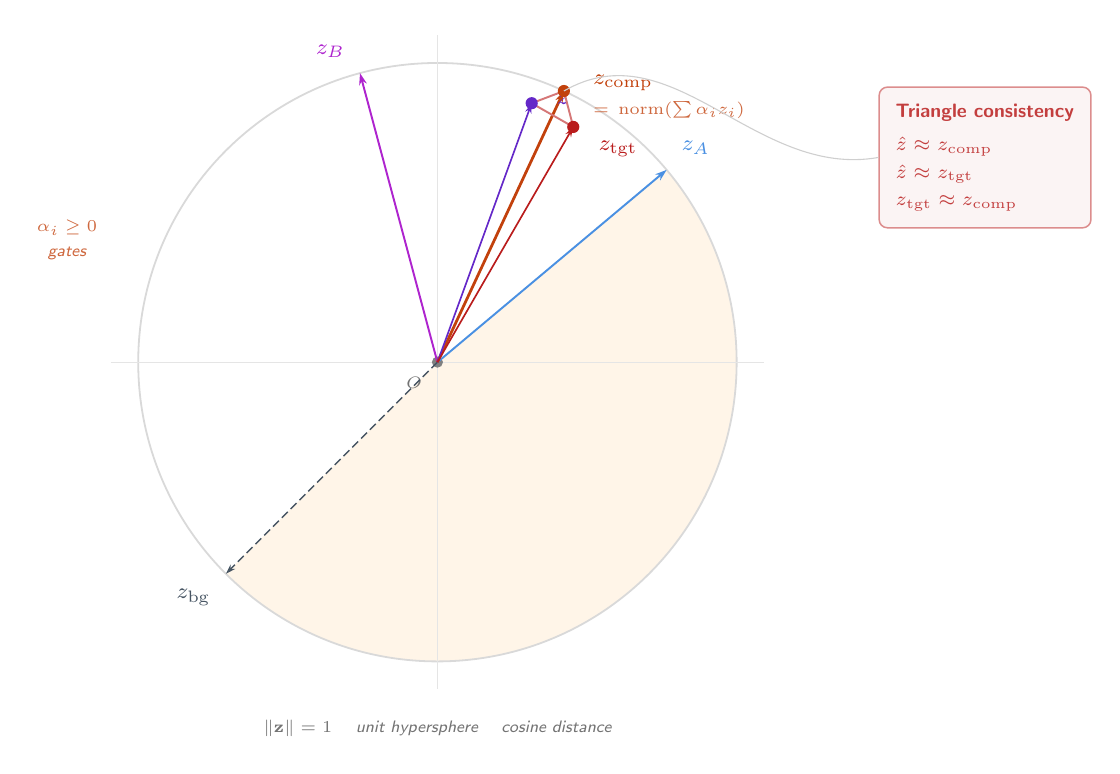
\begin{tikzpicture}[
  font=\small,
  >=Stealth,
  %% full-weight solid vector
  vec/.style={
    -{Stealth[length=4.2pt,width=2.8pt]}, line width=0.70pt
  },
  %% medium vector (predicted / target)
  vecm/.style={
    -{Stealth[length=3.6pt,width=2.3pt]}, line width=0.60pt
  },
  %% dashed vector (z_bg)
  vecd/.style={
    -{Stealth[length=3.6pt,width=2.3pt]}, line width=0.55pt,
    dashed, dash pattern=on 3pt off 1.5pt
  },
  ann/.style={
    font=\fontsize{8}{9.5}\selectfont\sffamily, align=center
  },
  lann/.style={
    font=\fontsize{6.5}{8}\selectfont\sffamily\itshape,
    text=black!55, align=center
  },
]

%% ── Geometry ─────────────────────────────────────────────────────────────────
\def\R{3.8}        % unit circle radius (cm)

\def\angA{40}      % z_A
\def\angB{105}     % z_B
\def\angBG{225}    % z_bg  (below-left)
\def\angComp{65}   % z_comp = norm(alpha_A z_A + alpha_B z_B + alpha_bg z_bg)
\def\angHat{70}    % z_hat  (slightly above z_comp)
\def\angTgt{60}    % z_tgt  (slightly below z_comp)

%% Slightly shorter radii for z_hat and z_tgt so their tips form a triangle
\def\Rhat{3.50}
\def\Rtgt{3.45}

%% ── Positive-cone fill (background layer) ────────────────────────────────────
%% Shaded from z_bg (225°) going counter-clockwise to z_A (40° = 400° equivalent)
\begin{scope}[on background layer]
  \fill[cCone, opacity=0.55]
    (0,0)
    -- ({\R*cos(\angBG)},{\R*sin(\angBG)})
    arc[start angle=\angBG, end angle=\angA+360, radius=\R]
    -- cycle;
\end{scope}

%% ── Unit circle ──────────────────────────────────────────────────────────────
\draw[gray!30, line width=0.65pt] (0,0) circle (\R);

%% Light reference axes
\draw[gray!20, line width=0.4pt] ({-\R-0.35},0) -- ({\R+0.35},0);
\draw[gray!20, line width=0.4pt] (0,{-\R-0.35}) -- (0,{\R+0.35});

%% Origin
\fill[black!50] (0,0) circle (2pt);
\node[lann, below left=2pt] at (0,0) {$O$};

%% ── Component vectors ─────────────────────────────────────────────────────────
%% z_A  (blue, solid)
\draw[vec, color=cA]
  (0,0) -- ({\R*cos(\angA)},{\R*sin(\angA)});
\node[ann, text=cA, above right=2pt]
  at ({\R*cos(\angA)},{\R*sin(\angA)}) {$z_A$};

%% z_B  (violet, solid)
\draw[vec, color=cB]
  (0,0) -- ({\R*cos(\angB)},{\R*sin(\angB)});
\node[ann, text=cB, above left=2pt]
  at ({\R*cos(\angB)},{\R*sin(\angB)}) {$z_B$};

%% z_bg (slate, dashed)
\draw[vecd, color=cEt]
  (0,0) -- ({\R*cos(\angBG)},{\R*sin(\angBG)});
\node[ann, text=cEt, below left=2pt]
  at ({\R*cos(\angBG)},{\R*sin(\angBG)}) {$z_{\mathrm{bg}}$};

%% ── z_comp (thicker, rust) ────────────────────────────────────────────────────
\draw[vec, color=cP1, line width=1.00pt]
  (0,0) -- ({\R*cos(\angComp)},{\R*sin(\angComp)});
%% label placed clearly to the right; scriptsize formula below
\node[ann, text=cP1, anchor=west]
  at ({\R*cos(\angComp)+0.25},{\R*sin(\angComp)+0.10})
  {$z_{\mathrm{comp}}$};
\node[font=\fontsize{6}{7}\selectfont\sffamily, text=cP1!80, anchor=west]
  at ({\R*cos(\angComp)+0.25},{\R*sin(\angComp)-0.24})
  {$=\,\mathrm{norm}(\textstyle\sum\alpha_i z_i)$};

%% ── z_hat (violet, medium, R_hat) ────────────────────────────────────────────
\draw[vecm, color=cP2]
  (0,0) -- ({\Rhat*cos(\angHat)},{\Rhat*sin(\angHat)});
\node[ann, text=cP2, anchor=west]
  at ({\Rhat*cos(\angHat)+0.20},{\Rhat*sin(\angHat)+0.08}) {$\hat{z}$};

%% ── z_tgt (crimson, medium, R_tgt) ──────────────────────────────────────────
\draw[vecm, color=cLo]
  (0,0) -- ({\Rtgt*cos(\angTgt)},{\Rtgt*sin(\angTgt)});
\node[ann, text=cLo, anchor=west]
  at ({\Rtgt*cos(\angTgt)+0.20},{\Rtgt*sin(\angTgt)-0.28}) {$z_{\mathrm{tgt}}$};

%% ── Triangle: z_comp -- z_hat -- z_tgt ───────────────────────────────────────
\coordinate (Pcomp) at ({\R*cos(\angComp)},    {\R*sin(\angComp)});
\coordinate (Phat)  at ({\Rhat*cos(\angHat)},  {\Rhat*sin(\angHat)});
\coordinate (Ptgt)  at ({\Rtgt*cos(\angTgt)},  {\Rtgt*sin(\angTgt)});

\draw[cLo!60, line width=0.70pt]
  (Pcomp) -- (Phat) -- (Ptgt) -- cycle;

%% vertex dots
\fill[cP1] (Pcomp) circle (2.2pt);
\fill[cP2] (Phat)  circle (2.2pt);
\fill[cLo] (Ptgt)  circle (2.2pt);

%% ── Triangle consistency callout box ─────────────────────────────────────────
%% Box placed far right at x >= 5.5 so it doesn't overlap vector labels
\node[
  rectangle, rounded corners=3pt,
  draw=cLo!50, line width=0.55pt, fill=cLo!5,
  inner sep=6pt,
  font=\fontsize{7}{9}\selectfont\sffamily,
  align=left, text=cLo!85,
  anchor=west
] (callout) at (5.60, 2.60)
{
  \textbf{Triangle consistency}\\[3pt]
  $\hat{z} \approx z_{\mathrm{comp}}$\\[1pt]
  $\hat{z} \approx z_{\mathrm{tgt}}$\\[1pt]
  $z_{\mathrm{tgt}} \approx z_{\mathrm{comp}}$
};

%% soft pointer line from Pcomp to callout
\draw[gray!38, line width=0.40pt]
  (Pcomp) to[out=30, in=190] (callout.west);

%% ── Gates / non-negative annotation  (left side) ─────────────────────────────
\node[lann, text=cP1!80, anchor=east]
  at ({-\R-0.40}, 1.55)
  {$\alpha_i \geq 0$\\[1pt]gates};

%% ── Bottom centre annotation ─────────────────────────────────────────────────
\node[lann] at (0,{-\R-0.85})
  {$\|\mathbf{z}\|=1$ \quad unit hypersphere \quad cosine distance};

\end{tikzpicture}
\end{document}
